\section{Study III: covariance-aware return bounds}\label{sec:window}
\subsection{A standard control for current deviation}
The noise-only obstruction motivates a control that averages noise while retaining a bound on current motion. This section states the assumptions explicitly, rather than interpreting a noisy empirical maximum as a model-error enclosure. For a dimensionless channel $j$, write
\begin{equation}
 e_{t,j}=v_{t,j}+\beta_{t,j}+\epsilon_{t,j},
 \qquad |\beta_{t,j}|\le B_j,\quad |v_{t,j}-v_{t-1,j}|\le L_j,
 \label{eq:decomposition}
\end{equation}
where $v$ is physical deviation from the nominal response, $\beta$ is reference bias, and $\epsilon$ is measurement noise. Assume a stationary zero-mean Gaussian AR(1) noise process with marginal standard deviation $\sigma_j$ and correlation $0\le\rho_j<1$. The variance of a mean over $m$ consecutive noise observations is
\begin{equation}
 V_{m,j}=\frac{\sigma_j^2}{m^2}
 \left[m+2\sum_{k=1}^{m-1}(m-k)\rho_j^k\right].
 \label{eq:covariance}
\end{equation}
Independence gives $V_{m,j}=\sigma_j^2/m$. Positive serial correlation reduces the effective averaging benefit.

Let $\mathcal M$ contain $K$ fixed windows, let $d$ be the number of channels, and allocate $\alpha_t=6\alpha/(\pi^2t^2)$ using a global clock that does not restart at alarms. Define
\begin{equation}
 U_{t,j}(m)=|\overline e_{t,j}(m)|+B_j
 +\sqrt{2V_{m,j}\log(2dK/\alpha_t)}
 +\frac{L_j(m-1)}{2}.
 \label{eq:windowbound}
\end{equation}
The last term is essential: a small window-average deviation need not imply a small deviation now.

\begin{proposition}
Under the stated Gaussian covariance, bias and increment assumptions, with probability at least $1-\alpha$, $|v_{t,j}|\le U_{t,j}(m)$ simultaneously for every channel, complete registered window and prospective time within a trace. Consequently, the decision
\begin{equation}
 \min_{m\in\mathcal M}U_{t,j}(m)\le\delta_j\qquad(j=1,\ldots,d)
 \label{eq:certificate}
\end{equation}
certifies coordinatewise return on that simultaneous event.
\end{proposition}
\begin{proof}
The Gaussian mean has variance $V_{m,j}$, so its two-sided tail at the square-root term in Equation~\ref{eq:windowbound} is at most $\alpha_t/(dK)$. Sum over channels, registered windows and times, using $\sum_{t=1}^{\infty}\alpha_t=\alpha$. Window overlap and cross-channel dependence do not invalidate this union bound. Finally, $|\overline\beta|\le B_j$ and
$|v_{t,j}-\overline v_{t,j}(m)|\le m^{-1}\sum_{k=0}^{m-1}kL_j=L_j(m-1)/2$.
The triangle inequality gives the result. Each coordinate may use a different minimizing window because all bounds hold simultaneously.
\end{proof}

This is an elementary comparison control, not a new time-uniform inference result. Its error allocation is conservative, and its validity depends on the supplied covariance and deterministic bounds. Unknown or invalid observations invalidate affected windows; they do not reset the clock. An absence of a certificate indicates uncertainty, not an attack alarm. The calculation does not model arbitrary colored, heavy-tailed or nonstationary noise.

\subsection{Prospective residual experiment}
The diagnostic fixes $d=4$, $\mathcal M=\{1,41,201\}$, $\alpha=0.05$, $\delta_j=0.1$ and $B_j=0.01$. Four $(\sigma,\rho)$ settings are $(0.03,0)$, $(0.06,0)$, $(0.03,0.8)$ and $(0.06,0.95)$, with channel standard-deviation multipliers $(1,0.8,1.1,0.9)$. For phases $\phi_j=(0,0.4,0.8,1.2)$, bias is $0.01\cos(0.003t+\phi_j)$. The physical-deviation signals are zero, $0.02\sin(0.004t+\phi_j)$, and $0.02\sin(0.04t+\phi_j)$, termed settled, slow and faster variation. They always lie within tolerance. The corresponding increment bound is $L_j=2a|\sin(\omega/2)|$, derived from the declared amplitude and frequency.

Each trace contains 1,200 samples, with the first noise value drawn from the stationary marginal. Seeds 17,42,2026 produce three independent innovation arrays reused across settings, giving 36 paired constructed traces rather than 36 independent acquisitions. The common reporting support is samples 201--1,200, or 1,000 endpoints per trace. The error statement is marginal per trace; no simultaneous 95\% guarantee across this whole matrix is claimed.

All four valid controls---the three fixed windows and their simultaneous envelope---receive identical residuals and parameter bounds. Two deliberately misspecified controls set $\rho=0$ for the 41- and 201-sample windows. Every variant and all 216 outcomes are retained. The criterion requires at least 95\% of common endpoints certified on every trace by the envelope. Parameters and conditions were recorded before generating outcomes; none was changed afterward.

These are synthetic residual signals, not outputs of the robot dynamics in Section~\ref{sec:simulation}. Noise, bias and increment bounds are known generator parameters. The experiment isolates their mathematical effects without establishing that those bounds are available from commissioning data. There is no attack, threshold fitting, model learning or measured post-attack recovery delay.

\subsection{Results and implications}
The envelope meets the criterion on 20 of 36 traces, so the overall normal-feasibility requirement fails. Table~\ref{tab:window} reports all condition groups, including seed ranges; Figure~\ref{fig:window} displays each group's worst seed. No instantaneous control endpoint is certified. Averaging restores normal certificates for several settings, but neither the longest window nor the assumption of independent noise is uniformly appropriate.

\begin{table}[htbp]\centering\small
\caption{Study III: simultaneous-envelope certificates on normal synthetic residuals. Each range spans the three seeds, each with 1,000 common endpoints. Passing requires at least 95\% on each trace.}\label{tab:window}
\setlength{\tabcolsep}{5pt}
\begin{tabular}{llrr}\toprule
Noise setting & Deviation profile & Certificates (\%) & Passes \\\midrule
Independent, low & Settled & 100.0--100.0 & 3/3 \\
Independent, low & Slow variation & 100.0--100.0 & 3/3 \\
Independent, low & Faster variation & 100.0--100.0 & 3/3 \\
Independent, high & Settled & 100.0--100.0 & 3/3 \\
Independent, high & Slow variation & 100.0--100.0 & 3/3 \\
Independent, high & Faster variation & 17.2--25.6 & 0/3 \\
Correlated, low & Settled & 100.0--100.0 & 3/3 \\
Correlated, low & Slow variation & 85.8--100.0 & 2/3 \\
Correlated, low & Faster variation & 0.0--0.0 & 0/3 \\
Correlated, high & Settled & 0.0--0.0 & 0/3 \\
Correlated, high & Slow variation & 0.0--0.0 & 0/3 \\
Correlated, high & Faster variation & 0.0--0.0 & 0/3 \\
\bottomrule\end{tabular}

\end{table}

\begin{figure}[htbp]\centering
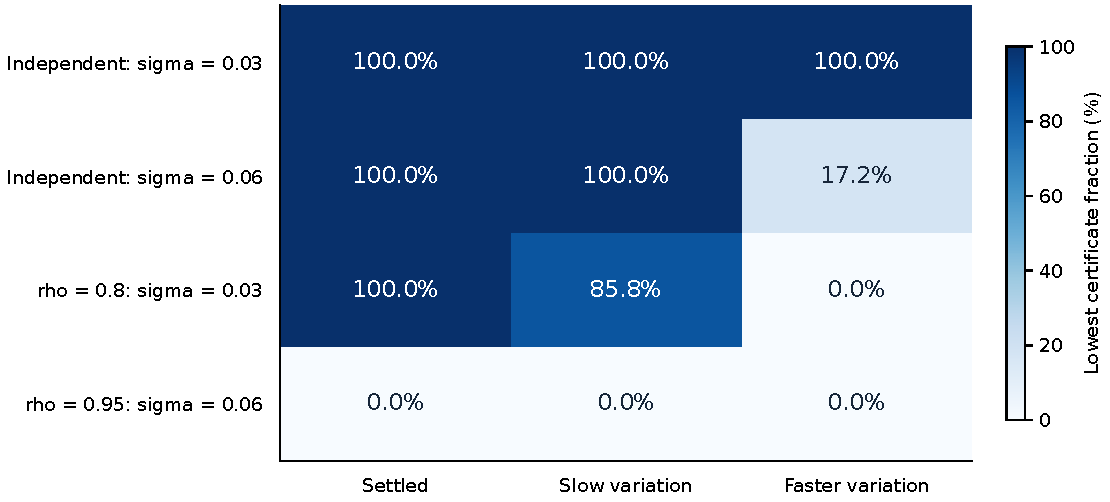
\includegraphics[width=0.88\linewidth]{figures/window_feasibility.pdf}
\caption{Lowest certificate fraction across seeds for each synthetic residual condition. All physical-deviation signals are within tolerance. A certificate establishes only the conditional bound in Equation~\ref{eq:certificate}; low coverage is not an attack-detection result.}\label{fig:window}
\end{figure}

For independent low noise with faster variation, window 41 certifies every endpoint, whereas window 201 certifies none. The longer window's drift allowance consumes its noise benefit. Under correlated low noise and slow variation, the envelope's fractions are 100\%, 85.8\% and 100\%: their 95.27\% average does not satisfy the all-traces criterion. At $\rho=0.95$ and $\sigma=0.06$, no valid control certifies any common endpoint, even for the settled profile. The misspecified 201-sample control would certify 91.53\% on average for that settled profile, but its uncertainty claim no longer follows from the actual covariance.

No coverage violation is observed in the within-tolerance traces. This is a numerical check under a constructed normal distribution, not an estimate of rare unsafe-clearing risk or evidence near the tolerance boundary. Longer averaging reduces the noise term while increasing the current-state variation term. A useful recovery mechanism must resolve that trade-off with justified information about noise and motion, rather than selecting the most favorable observed window after evaluation.

The diagnostic completed in 0.565 s wall time and 0.459 s CPU time, with 39.81 MiB sampled peak memory and 11.07 MiB of outputs. Twenty synthetic software checks and 2,665 saved-artifact checks support its implementation. These costs cover the entire small diagnostic and cannot be interpreted as robot deployment latency.
